\documentclass[border=10pt]{standalone}
\usepackage{tikz}
\usepackage{amsmath}
\usetikzlibrary{arrows.meta}

% ========== 配色定义 ==========
\definecolor{kwPos}{RGB}{222,240,222}  % 正权重背景（浅绿）
\definecolor{kwNeg}{RGB}{250,226,226}  % 负权重背景（浅红）
\definecolor{kwZero}{gray}{0.95}       % 0 权重背景（浅灰）

\begin{document}
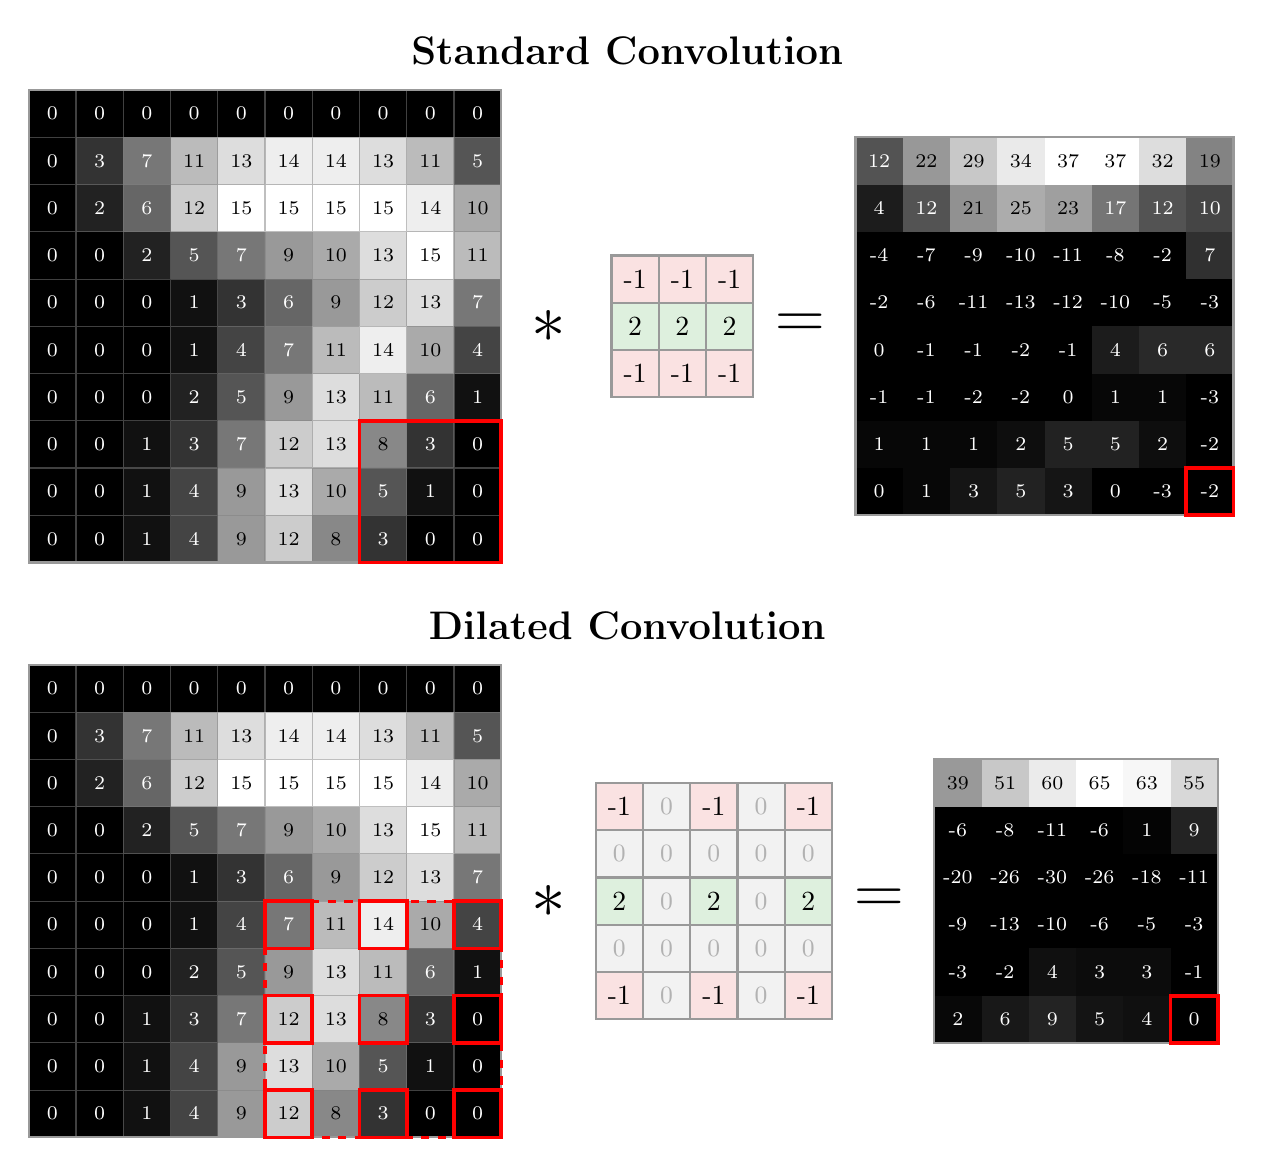
\begin{tikzpicture}[>={Stealth[length=4pt]}, line width=0.8pt, font=\large]

  % ========== 可复用：带数字的 10x10 图（格 0.6，#1 = y 偏移） ==========
  \newcommand{\drawimage}[1]{%
    \foreach \v [count=\n] in {%
      0,0,0,0,0,0,0,0,0,0,%
      0,3,7,11,13,14,14,13,11,5,%
      0,2,6,12,15,15,15,15,14,10,%
      0,0,2,5,7,9,10,13,15,11,%
      0,0,0,1,3,6,9,12,13,7,%
      0,0,0,1,4,7,11,14,10,4,%
      0,0,0,2,5,9,13,11,6,1,%
      0,0,1,3,7,12,13,8,3,0,%
      0,0,1,4,9,13,10,5,1,0,%
      0,0,1,4,9,12,8,3,0,0%
    }{%
      \pgfmathtruncatemacro{\col}{int(mod(\n-1,10))}
      \pgfmathtruncatemacro{\row}{int((\n-1)/10)}
      \pgfmathsetmacro{\gpct}{\v/15}
      \definecolor{px}{gray}{\gpct}
      \fill[px] ({0.6*\col}, {#1+0.6*(9-\row)}) rectangle ++(0.6,0.6);
      \ifnum\v>7 \def\tc{black}\else \def\tc{white}\fi
      \node[font=\scriptsize, text=\tc] at ({0.6*\col+0.3}, {#1+0.6*(9-\row)+0.3}) {\v};
    }
    \begin{scope}[shift={(0,#1)}]
      \draw[gray, opacity=0.5, thin, step=0.6] (0,0) grid (6,6);
      \draw[gray!80] (0,0) rectangle (6,6);
    \end{scope}
  }

  % ========== 可复用：标准 3x3 卷积核 ==========
  \newcommand{\drawkernel}[2]{%
    \foreach \w [count=\m] in {-1,-1,-1,2,2,2,-1,-1,-1} {%
      \pgfmathtruncatemacro{\kc}{int(mod(\m-1,3))}
      \pgfmathtruncatemacro{\kr}{int((\m-1)/3)}
      \ifnum\w>0
        \fill[kwPos] ({#1+0.6*\kc}, {#2+0.6*(2-\kr)}) rectangle ++(0.6,0.6);
      \else
        \fill[kwNeg] ({#1+0.6*\kc}, {#2+0.6*(2-\kr)}) rectangle ++(0.6,0.6);
      \fi
      \node[font=\normalsize] at ({#1+0.6*\kc+0.3}, {#2+0.6*(2-\kr)+0.3}) {\w};
    }
    \begin{scope}[shift={(#1,#2)}]
      \draw[gray!80, step=0.6] (0,0) grid (1.8,1.8);
      \draw[gray!80] (0,0) rectangle (1.8,1.8);
    \end{scope}
  }

  % ========== 可复用：空洞卷积核 5x5 (dilation r=2) ==========
  \newcommand{\drawdilatedkernel}[2]{%
    \foreach \w [count=\m] in {%
      -1,  0, -1,  0, -1,%
       0,  0,  0,  0,  0,%
       2,  0,  2,  0,  2,%
       0,  0,  0,  0,  0,%
      -1,  0, -1,  0, -1%
    } {%
      \pgfmathtruncatemacro{\kc}{int(mod(\m-1,5))}
      \pgfmathtruncatemacro{\kr}{int((\m-1)/5)}
      \ifnum\w>0
        \fill[kwPos] ({#1+0.6*\kc}, {#2+0.6*(4-\kr)}) rectangle ++(0.6,0.6);
        \node[font=\normalsize] at ({#1+0.6*\kc+0.3}, {#2+0.6*(4-\kr)+0.3}) {\w};
      \else\ifnum\w<0
        \fill[kwNeg] ({#1+0.6*\kc}, {#2+0.6*(4-\kr)}) rectangle ++(0.6,0.6);
        \node[font=\normalsize] at ({#1+0.6*\kc+0.3}, {#2+0.6*(4-\kr)+0.3}) {\w};
      \else
        \fill[kwZero] ({#1+0.6*\kc}, {#2+0.6*(4-\kr)}) rectangle ++(0.6,0.6);
        \node[font=\small, text=gray!60] at ({#1+0.6*\kc+0.3}, {#2+0.6*(4-\kr)+0.3}) {0};
      \fi\fi
    }
    \begin{scope}[shift={(#1,#2)}]
      \draw[gray!80, step=0.6] (0,0) grid (3.0,3.0);
      \draw[gray!80] (0,0) rectangle (3.0,3.0);
    \end{scope}
  }

  % ========== 可复用：8x8 结果灰度图（全填充） ==========
  \newcommand{\drawresultfull}[3]{%
    \foreach \v [count=\n] in {#3} {%
      \pgfmathtruncatemacro{\r}{int((\n-1)/8)}
      \pgfmathtruncatemacro{\c}{int(mod(\n-1,8))}
      \pgfmathsetmacro{\g}{max(0, min(\v/37, 1))}
      \definecolor{oc}{gray}{\g}
      \ifdim\g pt>0.5pt \def\tc{black}\else \def\tc{white}\fi
      \fill[oc] ({#1+0.6*\c}, {#2+0.6*(7-\r)}) rectangle ++(0.6,0.6);
      \node[font=\scriptsize, text=\tc] at ({#1+0.6*\c+0.3}, {#2+0.6*(7-\r)+0.3}) {\v};
    }%
    \draw[gray!80] (#1,#2) rectangle ({#1+4.8}, {#2+4.8});
  }

  % ========== 可复用：6x6 空洞卷积结果灰度图（全填充） ==========
  \newcommand{\drawdilatedresultfull}[3]{%
    \foreach \v [count=\n] in {#3} {%
      \pgfmathtruncatemacro{\r}{int((\n-1)/6)}
      \pgfmathtruncatemacro{\c}{int(mod(\n-1,6))}
      \pgfmathsetmacro{\g}{max(0, min(\v/65, 1))}
      \definecolor{oc}{gray}{\g}
      \ifdim\g pt>0.5pt \def\tc{black}\else \def\tc{white}\fi
      \fill[oc] ({#1+0.6*\c}, {#2+0.6*(5-\r)}) rectangle ++(0.6,0.6);
      \node[font=\scriptsize, text=\tc] at ({#1+0.6*\c+0.3}, {#2+0.6*(5-\r)+0.3}) {\v};
    }%
    \draw[gray!80] (#1,#2) rectangle ({#1+3.6}, {#2+3.6});
  }

  % =========================================================================
  % 第一行：标准卷积 (间隙减少 1/2，中心对齐至 y = 10.3)
  % =========================================================================
  \node[font=\bfseries\Large, anchor=center] at (7.6, 13.8) {Standard Convolution};

  % 输入图及右下角 3x3 感受野红框
  \drawimage{7.3}
  \draw[red, line width=1.4pt] (4.2, 7.3) rectangle (6.0, 9.1);

  \node[font=\Huge] at (6.6, 10.3) {$\ast$};

  % 3x3 卷积核
  \drawkernel{7.4}{9.4}

  \node[font=\Huge] at (9.8, 10.3) {$=$};

  % 8x8 完整结果
  \drawresultfull{10.5}{7.9}{%
    12,22,29,34,37,37,32,19,%
    4,12,21,25,23,17,12,10,%
    -4,-7,-9,-10,-11,-8,-2,7,%
    -2,-6,-11,-13,-12,-10,-5,-3,%
    0,-1,-1,-2,-1,4,6,6,%
    -1,-1,-2,-2,0,1,1,-3,%
    1,1,1,2,5,5,2,-2,%
    0,1,3,5,3,0,-3,-2}
  \draw[red, line width=1.4pt] ({10.5+0.6*7}, 7.9) rectangle ++(0.6,0.6);

  % =========================================================================
  % 第二行：空洞卷积 (中心 y = 3.0)
  % =========================================================================
  \node[font=\bfseries\Large, anchor=center] at (7.6, 6.5) {Dilated Convolution};

  % 输入图及右下角 5x5 跨度红虚线 + 9 个实际采样格实线红框
  \drawimage{0}
  \draw[red, dashed, line width=1.1pt] (3.0, 0.0) rectangle (6.0, 3.0);
  \foreach \c in {5,7,9} \foreach \r in {0,2,4} {
    \draw[red, line width=1.3pt] ({0.6*\c}, {0.6*\r}) rectangle ++(0.6,0.6);
  }

  \node[font=\Huge] at (6.6, 3.0) {$\ast$};

  % 5x5 空洞卷积核
  \drawdilatedkernel{7.2}{1.5}

  \node[font=\Huge] at (10.8, 3.0) {$=$};

  % 6x6 完整结果
  \drawdilatedresultfull{11.5}{1.2}{%
     39,  51,  60,  65,  63,  55,%
     -6,  -8, -11,  -6,   1,   9,%
    -20, -26, -30, -26, -18, -11,%
     -9, -13, -10,  -6,  -5,  -3,%
     -3,  -2,   4,   3,   3,  -1,%
       2,   6,   9,   5,   4,   0}
  \draw[red, line width=1.4pt] ({11.5+0.6*5}, 1.2) rectangle ++(0.6,0.6);

\end{tikzpicture}
\end{document}